\documentclass{standalone}

\usepackage{circuitikz}

\begin{document}

% INT_AY21_L33_Fig06_Q_vs_V_graph.png

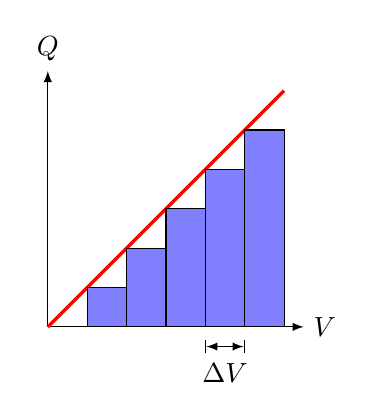
\begin{tikzpicture}[> = latex]

	% Axes
	
	\draw [<->] (0, 3.25) node [above] {$Q$} -- (0, 0) -- (3.25, 0) node [right] {$V$};
	
	% Graph curve
	
	\draw [very thick, red] (0, 0) -- (3, 3);
	
	% Rectangles
	
	\foreach \x in {0.5, 1, ..., 2.5}
		\filldraw [blue!50, draw = black] (\x, 0) rectangle ({\x + 0.5}, \x);
		
	\draw [|<->|] (2, -0.25) -- node [below = 0.25 em] {$\Delta V$} (2.5, -0.25);

\end{tikzpicture}


\end{document}